\section{Розробка, навчання та тестування програмного забезпечення}
\subsection{Особливості програмної реалізації системи, що розробляється}
Для розробки програмної системи була використані мова програмування Python та застосовані патерни проектування типу GoF та принципи Сlean architecture~\cite{Martin2017}.

\subsection{Навчання програмної системи}
\subsubsection{Генерація даних для навчання}
Для генерації даних було написано програму, яка зберігає поточні точки обличчя користувача та поточну позицію курсора на екрані користувача.

Таким шляхом було згенеровано дві тисячі прикладів для навчання нейронної мережі.

Скрипт для генерації представлено у додатках.

\subsubsection{Навчання моделі}
Було проведено 200 ітерацій навчання моделі: 
\begin{lstlisting}
model.compile(loss='binary_crossentropy', optimizer='adam', metrics=['mean_squared_error'])
model.fit(np.array(X), np.array(Y), epochs=200, verbose=1)
\end{lstlisting}

Динаміка середньоквадратичної помилки зображена на рисунку~\ref{fig:results_training}.
На рисунку видно, що результати мережі не сильно покращуються починаючі з 80 епохи навчання. 

\begin{figure}[H]
    \centering
  \begin{tikzpicture}
    \begin{axis}[ 
      xlabel={Епоха},
      ylabel={Помилка},
      xmin=0,xmax=200,ymin=0,ymax=10000
    ] 
      \addplot
          coordinates {
              (0,9853) [0]
              (20,3214) [1]
              (40,704) [2]
              (60,83) [3]
              (80,43) [4]
              (100,14) [5]
              (120,9) [6]
              (140,2) [7]
              (160,0.7) [8]
              (200,0.6) [9]
          };
    \end{axis}
  \end{tikzpicture}
  \caption{Динаміка середньоквадратичної помилки}
  \label{fig:results_training}
\end{figure}

\subsection{Тестування програмної системи}
\subsubsection{Ручне тестування}
Було проведено ручне тестування, та визначено, що програмна система достатньо добре визначає приблизну область, в яку дивиться користувач (рисунок~\ref{fig:test_1}).

\begin{figure}[H]
	\centering
	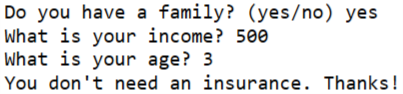
\includegraphics[width=0.6\textwidth]{test_1}
	\caption{Передбачення погляду}
	\label{fig:test_1}
\end{figure} 

Було визначено, що програма гірше передбачує точки на межах області монітору (рисунок~\ref{fig:test_2}), що пояснюється використанням сігмоїди у останньому шарі нейронної мережі.

\begin{figure}[H]
	\centering
	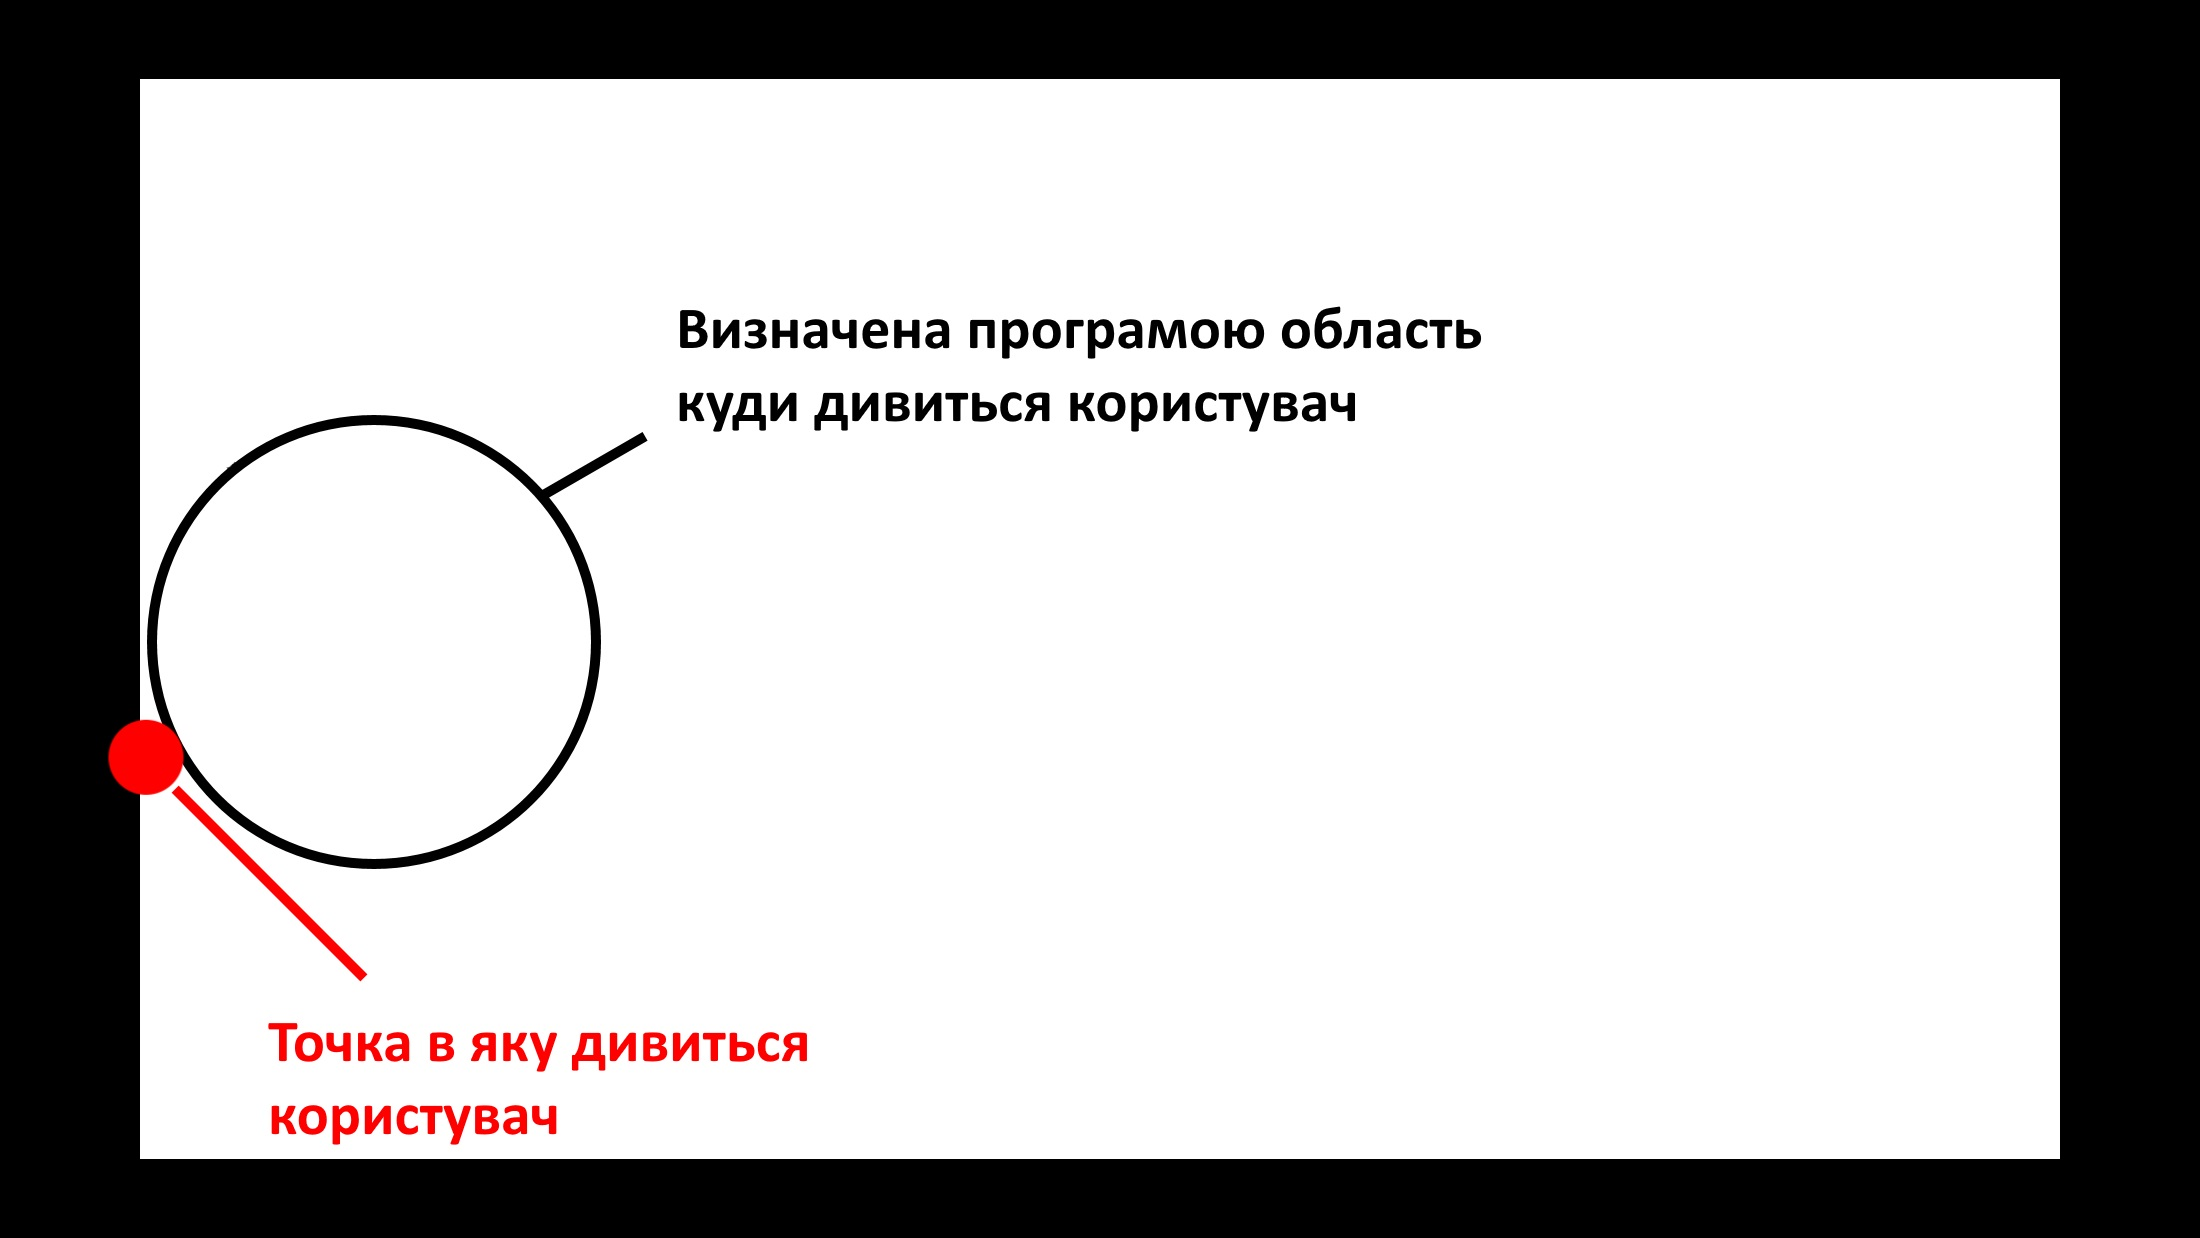
\includegraphics[width=0.6\textwidth]{test_2}
	\caption{Передбачення погляду на межі монітору}
	\label{fig:test_2}
\end{figure} 

Інтерфейс керування курсором зображено на рисунку~\ref{fig:cursor}.

\begin{figure}[H]
	\centering
	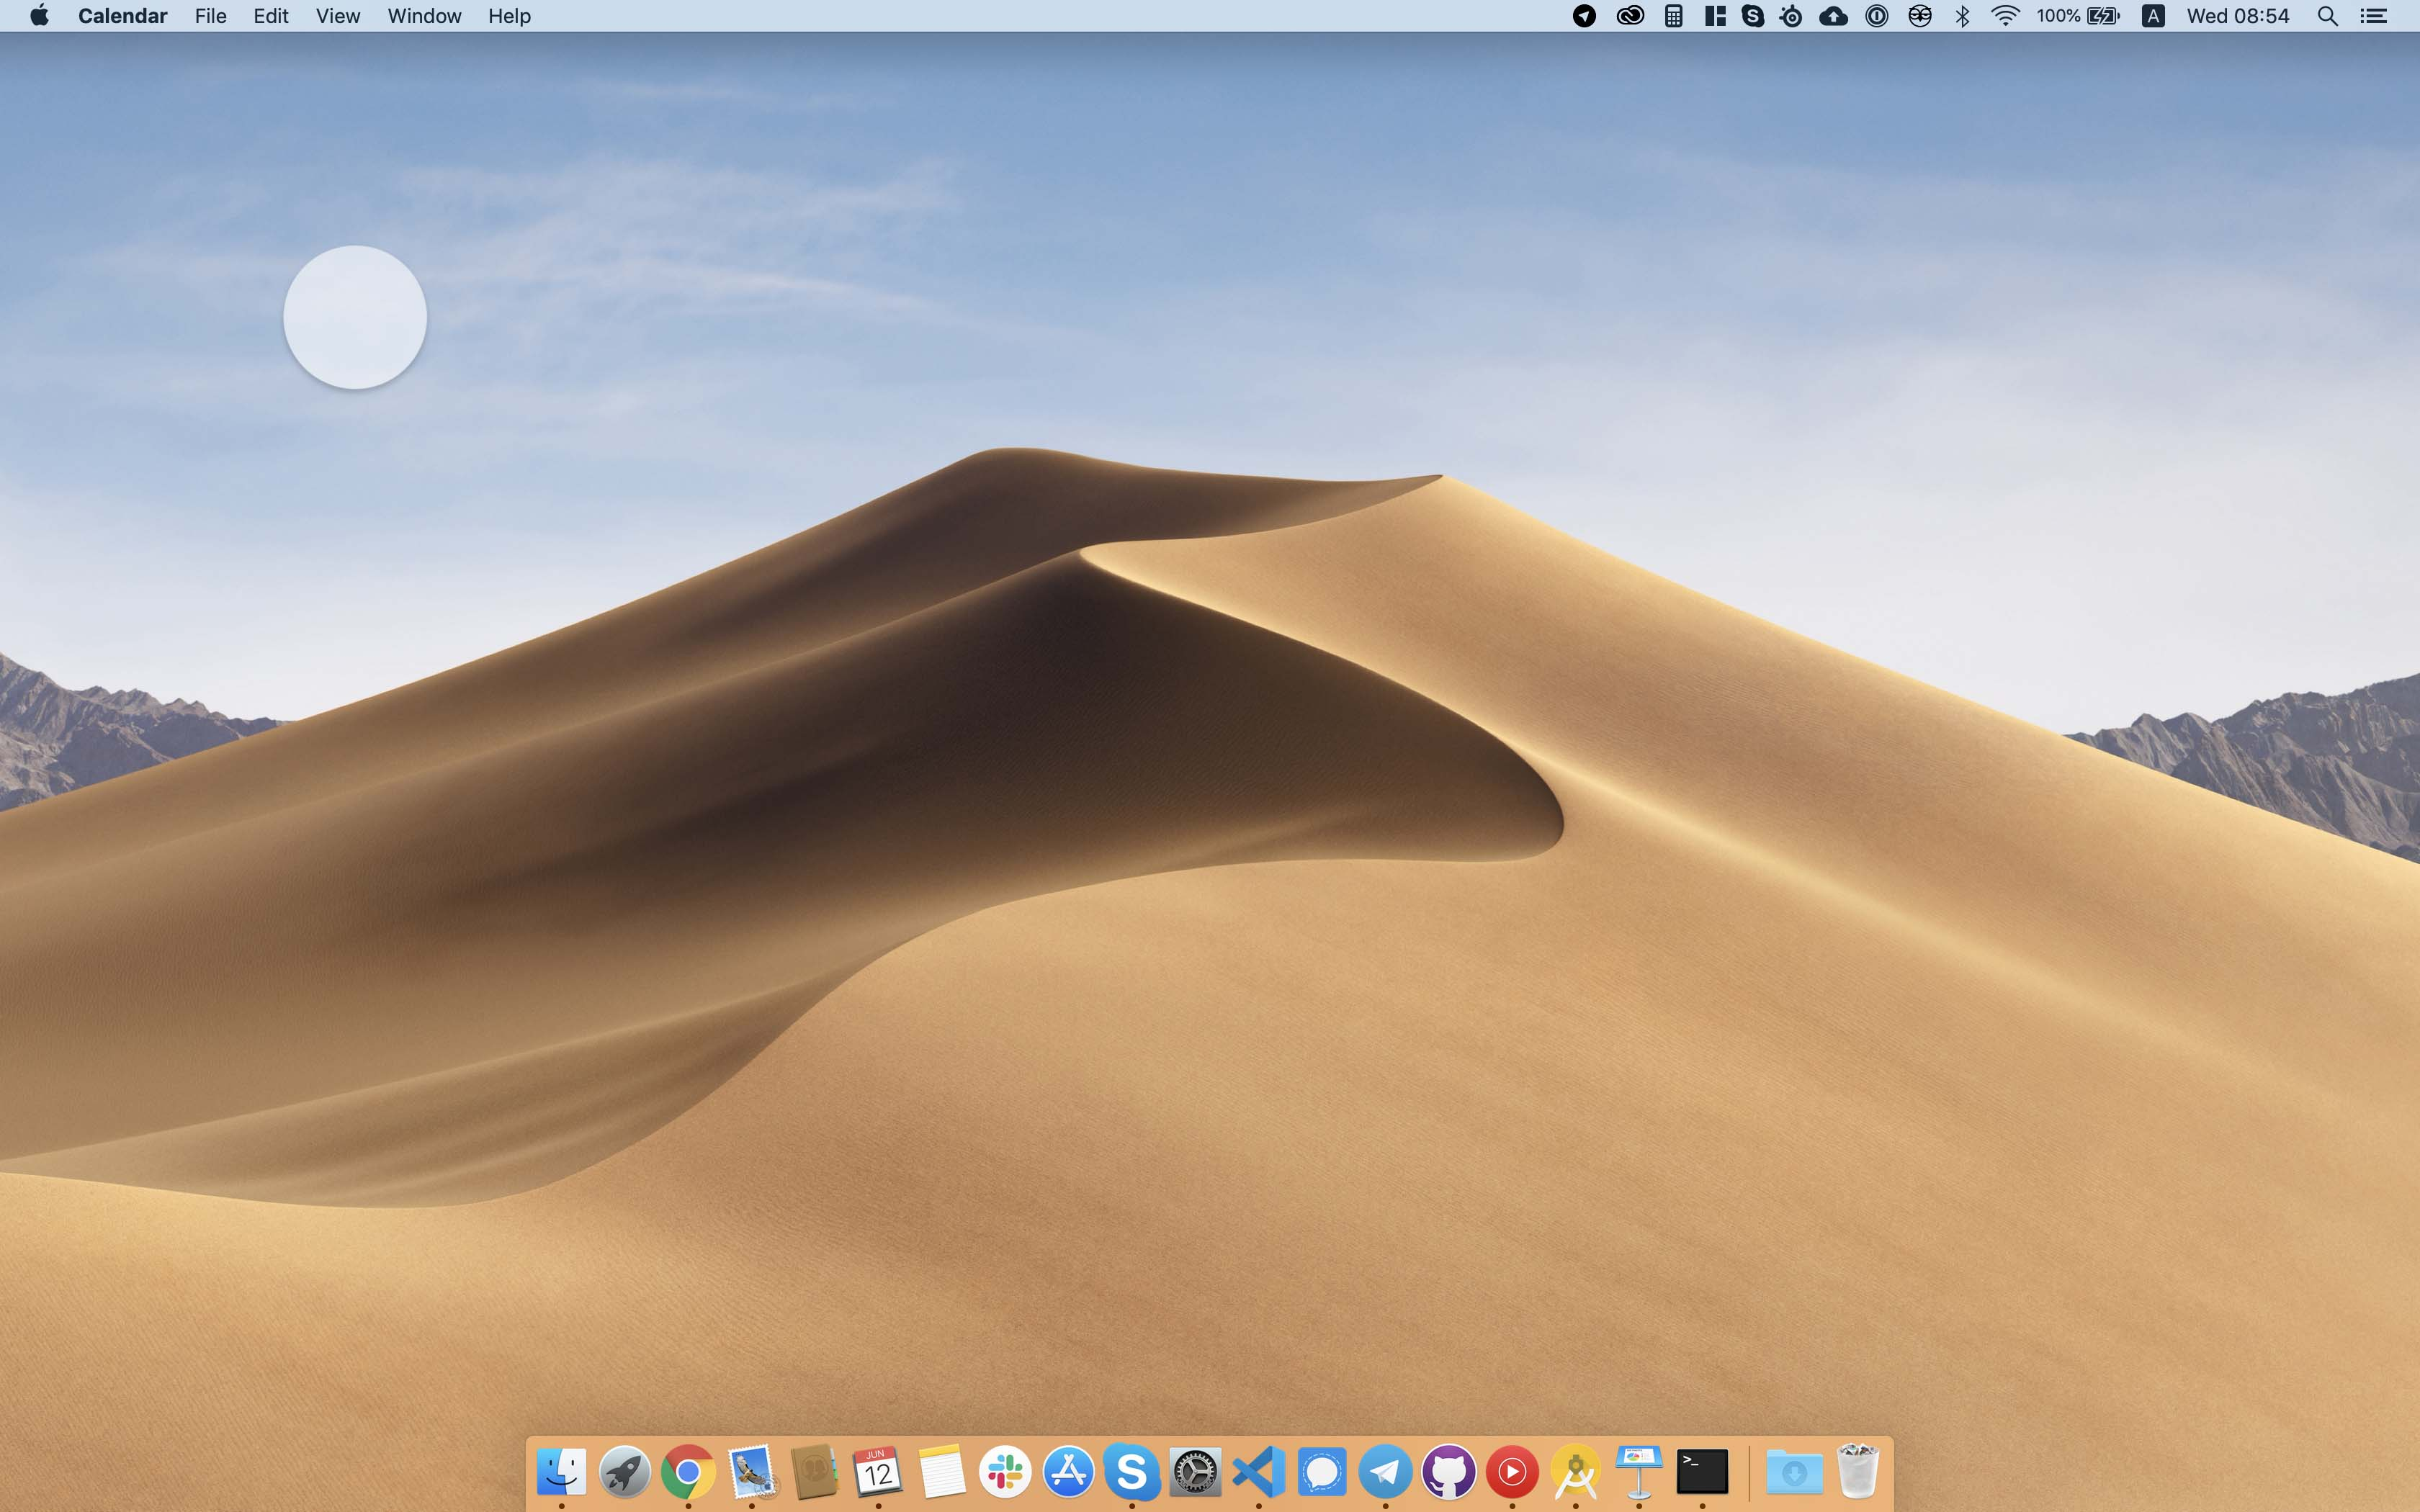
\includegraphics[width=0.6\textwidth]{screen}
	\caption{Керування курсором}
	\label{fig:cursor}
\end{figure} 

\subsubsection{Середньоквадратична помилка}
Для перевірки середньоквадратичної помилки початкові дані були розбиті у пропорціях 8:2 на дані для навчання та данні для тестування.

Було проведено 200 ітерацій навчання моделі.

Середньоквадратична помилка є $e = 0.584$, що робить таку систему пригодну для прикладного використання.
